\chapter{Návrh}
\label{kap:nav}

\section{Funkcie aplikácie}
Ako sme si mohli všimnúť v \ref{sec:applications}, všetky aplikácie ponúkajú vyhľadávanie z aktuálnej polohy rovnako ako aj možnosť výberu zastávky priamo z mapy. Tieto funkcie bude používateľovi ponúkať aj naša aplikácia. Väčšina spomenutých aplikácií ponúkala zobrazenie histórie vyhľadávania, ktorá odľahčí používateľa od zadávania parametrov v prípade, že vyhľadáva väčšinou tie isté spoje. Túto funkcionalitu nájde používateľ aj v našej aplikácii. História vyhľadávania sa bude ukladať do pamäte zariadenia. 

Okrem aplikácie \textit{UBIAN} a \textit{CP} si používatelia vedia zobraziť všetky linky v MHD a postupnosti zastávok, ktoré obsluhujú. Túto funkciu bude ponúkať aj naša aplikácia. Čo sa týka nastavenia prídavných preferencií pri vyhľadávaní, aplikácie ponúkajú rôzne preferencie. Najčastejšími z nich sú: maximálny počet prestupov, minimálny čas na prestup, limit pre peší presun a  zobrazenie len nízkopodlažých vozidiel. Naša aplikácia bude mať možnosť nastavenia všetkých týchto preferencií.

Jediná aplikácia, ktorá ponúka informácie o reálnom pohybe vozidiel vo forme meškania, je aplikácia \textit{UBIAN}. Predpokladáme však, že aj táto aplikácia vyhľadáva v statických cestovných poriadkoch a pri vyhľadanom spoji len pripíše informáciu vo forme meškania. Uvažujeme tak na základe toho, že po vyhľadaní spojov zo zastávky po zadaní aktuálneho času aplikácia ponúkne také spoje, ktoré podľa statických cestovných poriadkov majú na túto zastávku v blízkej budúcnosti príchod. Ak existuje taký spoj, ktorý mal odchod z danej zastávky v minulosti, ale má meškanie a na zastávke ešte nebol, aplikácia ho nezobrazí.V tomto prípade naša aplikácia ponúkne aj tie spojenia, ktoré kvôli meškaniu na zastávku ešte nedorazili. Pre vyhľadaný spoj zobrazí  čas odchodu zo statických dát cestovného poriadku a pripíše k nemu informáciu o  meškaní.

Medzi ďalšie funkcionality patrí zakúpenie lístka priamo cez aplikáciu. Táto funkcionalita však nesúvisí priamo s našim zadaním a navyše je potrebná zmluva s dopravcami. Preto naša aplikácia túto možnosť ponúkať nebude.

Aplikácia \textit{Imhd.sk} a \textit{CG Tranzit} fungovali aj v offline režime. Hoci je užitočné ponúknuť vyhľadávanie bez možnosti prístupu na internet, znamenalo by to že náš algoritmus by bežal na klientskej strane.  Keďže hlavnou úlohou našej aplikácie je vyhľadávanie spojov z reálnych dát, aplikácia bude fungovať online s tým, že zaručí používateľom, vždy aktuálne spojenia. 

V tabuľke \ref{table:aplication-funcions} je zobrazený prehľad funkcionalít našej navrhovanej aplikácie a iných existujúcich aplikácii na vyhľadávanie spojov v MHD Bratislava.

\begin{table}[H]
\footnotesize
\begin{tabular}{|L{4.49cm}|c|c|c|C{1.29cm}|c|C{1.54cm}|}
\hline
\rowcolor[HTML]{C0C0C0} 
\textbf{} & \textbf{Imhd.sk} & \textbf{IDS BK} & \textbf{CP} & \textbf{CG Tranzit} & \textbf{UBIAN} & \textbf{Naša aplikácia}
\\ \hline
\textbf{z aktuálnej polohy} & \cmark & \cmark  & \cmark  & \cmark  & \cmark  & \cmark    
\\ \hline
\textbf{výber zástavok z mapy} & \cmark & \cmark  & \cmark  & \cmark  & \cmark & \cmark       
\\ \hline
\textbf{história vyhľadávania} & \cmark & \xmark  & \cmark  & \cmark  & \cmark & \cmark         
\\ \hline
\textbf{zobrazenie liniek} & \cmark & \cmark  & \xmark  & \cmark  & \xmark & \cmark         
\\ \hline
\textbf{max. počet prestupov} & \cmark & \cmark  & \cmark  & \cmark  & \xmark & \cmark         
\\ \hline
\textbf{min. čas na prestup} & \cmark & \xmark  & \cmark  & \cmark  & \xmark & \cmark         
\\ \hline
\textbf{limit pre peší presun} & \cmark & \cmark  & \xmark  & \xmark  & \xmark  & \cmark        
\\ \hline
\textbf{len nízkopodlažné vozidlá} & \cmark & \xmark  & \cmark  & \xmark  & \xmark  & \cmark        
\\ \hline
\textbf{meškanie MHD} & \xmark & \xmark  & \xmark  & \xmark  & \cmark & \cmark         
\\ \hline
\textbf{kúpa lístkov} & \xmark & \cmark  & \cmark  & \cmark  & \cmark & \xmark         
\\ \hline
\textbf{offline režim} & \cmark & \xmark  & \xmark  & \cmark  & \xmark  & \xmark        
\\ \hline
\end{tabular}
\caption{Tabuľka funkcionalít existujúcich aplikácií a navrhovanej aplikácie}
\label{table:aplication-funcions}
\end{table}


\section{Architektúra aplikácie}

Klient sa bude dopytovať na server pre vyhľadanie spojenia. Server spustí výpočet nad dátovou štruktúrou, ktorá má aktuálne cestovné poriadky s aktuálnymi odchodmi spojov a vráti odpoveď klientovi.

Algoritmus bude pracovať nad dátovou štruktúrou, ktorá bude obsahovať stále aktuálne dáta. Dátová štruktúra bude uložená na serverovej strane. 

\subsection{Serverová strana}
Na serverovej strane bude bežať aplikačný server \textit{Tomcat}. Na uchovanie dát použijeme relačnú databázu \textit{PostgreSQL}. Jazyk, v ktorej bude aplikácia implementovaná je \textit{Java 11}.
 
Na mapovanie java objektov na tabuľky databázy použijeme ORM framework \textit{Hibernate}. \textit{Hibenate} zároveň ponúka implementáciu \textit{Java Persistnace API}. 

Na komunikáciu s klientom budeme používať \textit{REST API}. Na vytvorenie RESTových webových služieb použijeme na serverovej strane \textit{Spring} framework. Na špecifikáciu \textit{REST API} použijeme \textit{Swagger }framework. API budeme popisovať v \textit{JSON} súbore. 

\subsection{Klientská strana}
Na klientskej strane sme sa rozhodli pre progresívnu webová aplikácia \textit{PWA}. Je to webová aplikácia, ktorá sa dokáže správať ako mobilná aplikácia, ktorá sa neustále aktualizuje, pričom nie je potrebná jej inštalácia. Po návšteve webovej stránky na mobilnom zariadení, používateľ dostane upozornenie od stránky, či si ju chce uložiť do zariadenia ako mobilnú aplikáciu. Progresívna webová aplikácia zaberá minimum miesta v pamäti a má svoj vlastný úložný priestor, kde sa budú ukladať preferencie a história vyhľadávania.
Na implementáciu použijeme moderný JavaScriptový framework \textit{VUE.js}.

\subsection{Spracovanie dát (zatiaľ 2 verzie)}
\subsubsection{Verzia 1. Ak budú dostupné reálne dáta + statické dáta pre jednotný cestovný poriadok}
Pri spustení aplikácie alebo po aktualizácii cestovných poriadkov sa spustí služba, ktorá nám z úložiska, kde sú aktuálne cestovné poriadky namapuje dáta do našej databázy. Po tom ako budú dáta uložené v databáze sa spustí ďalšia služba, ktorá obnoví dátovú štruktúru podľa nových cestovných poriadkov. Táto služba sa zároveň bude spúšťať na prelome dní, pretože cez sviatky a víkendy jazdia iné linky ako v bežný pracovný deň a teda aj dátová štruktúra bude vyzerať inak.
 
Server bude komunikovať s databázou, ktorá zaznamenáva aktuálne odchody vozidiel zo zastávok alebo nejakým snapshotom tejto databázy. Medzi nimi bude služba, ktorá bude mať na starosti zaznamenávať reálne odchody spojov do dátovej štruktúry. 

Spôsob akým bude aplikácia nasadená je znázornená na obrázku \ref{fig:deploymentDiagram}.

\subsubsection{Verzia 2. Ak bude treba vytvoriť testovaciu sadu a simulovať reálnu dopravnú situáciu}
Statické dáta jednorazovo získame preparsovaním webovej stránky iMHD.sk a uložíme ich do našej databázy. 

Pri spustení aplikácie sa spustí služba, ktorá vytvorí dátovú štruktúru pre algoritmus na serveri a naplní ju údajmi z databázy. Táto služba sa bude spúšťať aj na prelome dní, pretože cez sviatky a víkendy jazdia iné linky ako v bežný pracovný deň a teda aj dátová štruktúra bude vyzerať inak. 

Reálnu dopravnú situáciu môžeme simulovať viacerými spôsobmi:
\begin{itemize}
\item{Pre každý spoj a pre každý odchod z každej zastávky vytvoríme údaj vo forme (čas, spoj, zastávka). Tento spôsob je namáhavejší, ale zrejme sa viac podobá reálnym dátam. }
\item{Reagovať budeme len na meškanie. Vytvoríme záznamy len pre meškanie spoja (spoj, meškanie - od, do, koľko).}
\end{itemize}

Vytvoríme službu, ktorá bude prechádzať takéto záznamy a meniť údaje o odchodoch spojov v dátovej štruktúre.

\begin{figure}[H]
\centerline{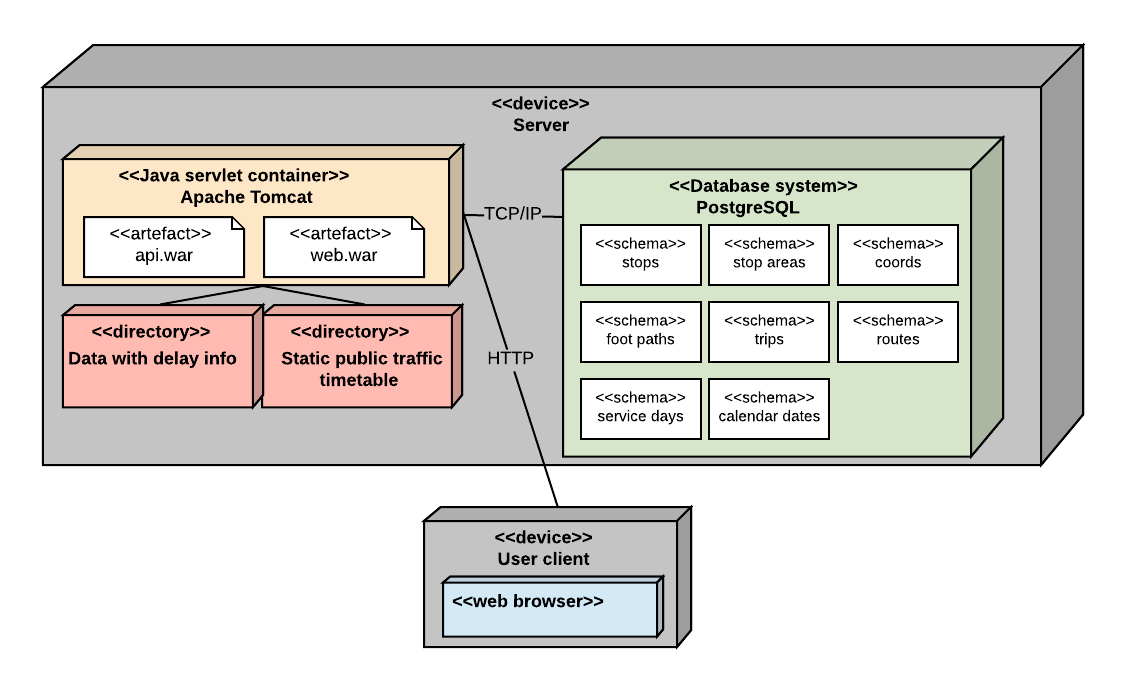
\includegraphics[width=1.0\textwidth]{images/deployment-diagram}}
\caption[Diagram nasadenia]{Diagram nasadenia)}
\label{fig:deploymentDiagram}
\end{figure}

\section{Algoritmus}
Pri hľadaní algoritmu na nájdenie optimálnej cesty sme najskôr siahli po najznámejšom vyhľadávacom grafovom algoritme. Dijkstrov algoritmus sa zdal vhodný, avšak jeho vylepšená verzia A* algoritmus je pri správne zvolenej heuristike efektívnejšia. Keďže zastávky, ktoré predstavujú vrcholy v grafe majú dané súradnice, môžeme pri vyhľadávaní optimalizovať prehľadávaný priestor. Pri štúdiu článkov sme narazili na rôzne optimalizácie, ktoré sú spomenuté v \ref{sec:optimalization}.

V prípade cestovných poriadkov je náročné správne namodelovať graf, ktorý dokáže efektívne spracovať časovo závislé dáta. V \ref{sec:models} boli spomenuté dva overené prístupy \textit{Time dependent} a \textit{Time expanded model}, ktoré tento problém riešia. 

Ďalšou výzvou je prispôsobiť algoritmus, aby dokázal vypočítať najoptimálnejšiu cestu, (príp. viacero optimálnych ciest) s ďalšími pridanými kritériami. Kvôli dynamickej povahe verejnej dopravy, grafový prístup v kombinácii s vyhľadávacím grafovým algoritmom vyžaduje veľa pre-processingu. Výhodou vo verejnej doprave je, že vozidlá sa pohybujú po vyznačených linkách, ktorých trasy poznáme. Schéma verejnej dopravy sa preto dá zachytiť do pomerne jednoduchých dátových štruktúr. Tento fakt si všimli aj autori algoritmu RAPTOR, ktorý sme opísali v \ref{sec:raptor}. 

V našej aplikácii sme sa rozhodli použiť tento negrafový algoritmus. Využijeme základnú verziu RAPTOR algoritmu popísanú v \ref{sub:raptor-basic} a súčasne využijeme aj jeho optimalizáciu opísanú v \ref{sub:raptor-optimalisation}, kedy označujeme zastávky, aby sme nemuseli prechádzať tie linky, ktorým sa nevylepšil čas $\tau_{k-1}(p)$. Optimalizáciu \textit{local-prunning} nevyužijeme, keďže chceme použiť rozšírenú verziu RAPTOR algoritmu a to je rRAPTOR algoritmus popísaný v sekcii \ref{sub:rraptor}. Algoritmus rRAPTOR nám nevráti len jednu najkratšiu cestu, ktorá začína najskôr od zadaného času, ale vráti nám množinu najkratších ciest, začínajúcich v zadanom časovom úseku.

Cesta, ktorú nám vráti základná verzia RAPTOR algoritmu je najkratšia a nezáleží koľko prestupov bude obsahovať. Našou úlohou je používateľovi poskytnúť optimálnu cestu a keďže optimálna cesta môže byť pre každého používateľa iná, ponúkneme mu viacero alternatív.  Túto funkciu ponúka vylepšený RAPTOR algoritmus popísaný v \ref{sec:raptor-improved}. Algoritmus nám vráti viacero optimálnych ciest, pričom prihliada na to, aby jednotlivé cesty neboli rovnaké na veľkej časti úseku.

Našim cieľom je zlúčiť rRAPTOR algoritmus s vylepšeným RAPTOR algoritmom na hľadanie viacerých ciest a zakomponovať mechanizmus, schopný zohľadniť zadané používateľské preferencie, ktoré bude algoritmus prijímať ako vstupné parametre. Preferencie, ktoré bude vedieť algoritmus zohľadniť: minimálny čas na prestup, maximálny počet prestupov, maximálna dĺžka pešieho prestupu a vyhľadanie len nízkopodlažných spojov. 

Výstupom z nášho algoritmu bude množina ciest, začínajúcich na zastávke $p_s$, po čase $\tau$ a končiacich v zastávke $p_t$. Jednotlivé cesty sú optimálne, vyhovujú prípadným používateľským preferenciám a ich časy odchodov sú z časového intervalu <$\tau, \tau + \Delta \tau$>. 

Ak používateľ zadá ako začiatočnú zastávku aktuálnu polohu, nájdeme zastávky v okolí radiálnym vyhľadávaním, ako bolo spomenuté v \ref{sec:actual-location}. Najbližšia vyhľadaná zastávka k aktuálnemu bodu nemusí znamenať optimálne riešenie a preto budeme považovať za začiatočnú zastávku každú z nich. Pre každú zastávku zvlášť spustíme algoritmus, ktorý nám pre každú z nich vráti množinu optimálnych ciest a na záver z nich vyberieme $n$ najoptimálnejších ciest. Do finálneho riešenia zakomponujeme peší presun od aktuálnej polohy po začiatočnú zastávku vybraných optimálnych ciest.

\section{Dátová štruktúra}
Rovnako dôležitý je dobre navrhnutá dátová štruktúra, s ktorou bude algoritmus vedieť rýchlo a efektívne pracovať. Budeme sa inšpirovať dátovou štruktúrou z \ref{subsec:structure}, ktorá bola navrhnutá pre základnú verziu RAPTOR algoritmu. Dátová štruktúra bude obsahovať aktuálne cestovné poriadky s prispôsobenými príchodmi a odchodmi vozidiel podľa prípadných meškaní.  

\section{Dáta}
Pri vývoji aplikácie a pre jej testovanie sú nevyhnutné dáta. Pre účely aplikácie budeme potrebovať dáta zo statických cestovných poriadkov a dáta o aktuálnych pozíciách jednotlivých vozidiel. Faktom je, že potrebujeme reálne a statické dáta z obdobia, keď boli cestovné poriadky rovnaké. 

...........

(Cestovné poriadky pre MHD BA sú k dispozícii na voľné stiahnutie na stránke INPROP.sk. Sú však určené len pre aplikáciu \textit{Cestovné Poriadky} na vyhľadávanie spojov, ktorá ich vie spracovať. Táto aplikácie je stiahnuteľná za poplatok. So súborom sa nedá pracovať, pretože je v Text Template formáte, ktorý je určený len pre kontrétnu aplikáciu, ktorá ho používa. 

...........

\section{Databáza}

Na serveri budú uložené dáta aplikácie v PostgreSQL databáze. Databáza sa naplní pri prvotnom spustení aplikácie na serveri a v prípade, kedy dostaneme upozornenie na aktualizáciu statických poriadkov. Schéma databázy je popísaná entitno-relačným diagramom na obrázku \ref{fig:erd}.

\begin{figure}[H]
\centerline{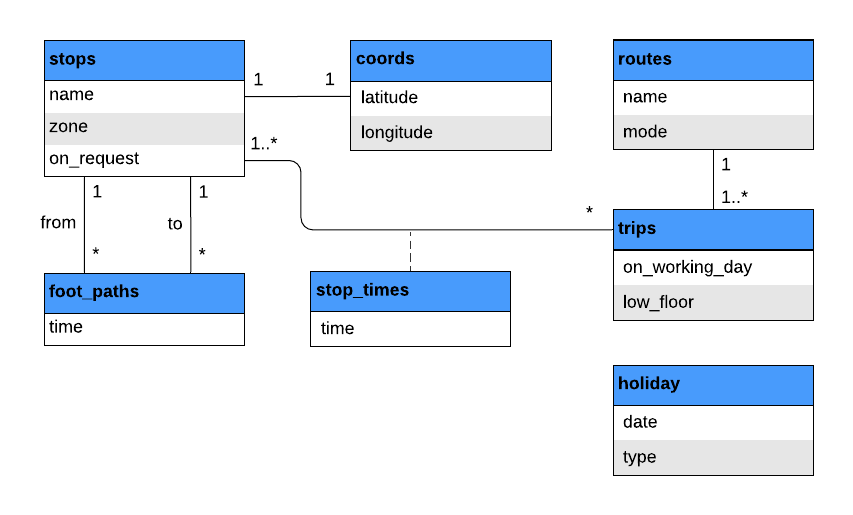
\includegraphics[width=1.0\textwidth]{images/ERD}}
\caption[Entitno-relačný diagram]{Entitno-relačný diagram}
\label{fig:erd}
\end{figure}

V entite \textit{stops} evidujeme názov zastávky (\textit{name}), zónu mesta (\textit{zone}), do ktorej zastávka patrí a hodnotu \textit{on\_request}, ktorá udáva, či je zastávka na znamenie. Každá zastávka má súradnice, ktoré sa udržujú v entite \textit{coords}.

V entite \textit{coords} sú súradnice určené atribútmi zemepisná šírka (\textit{latitude}) a zemepisná výška (\textit{longitude}). 

Entita \textit{foot\_paths} obsahuje atribút \textit{time}, ktorý určuje čas potrebný na peší presun zo zastávky \textit{from} na zastávku \textit{to}.

V entite \textit{routes} sa udržuje zoznam liniek, jazdiacich aktuálne v bratislavskej hromadnej doprave. Linka je určená názvom (\textit{name}) a módom (\textit{mode}). V Bratislave jazdia 3 rôzne módy: električka, trolejbus a autobus. Každá linka má počas dňa viaceré jazdy (\textit{trips}).

Entita (\textit{trips}) uchováva informáciu o tom, či je vozidlo, ktoré bolo pridelené konkrétnej jazde nízkopodlažné a zároveň či jazda linky premáva počas pracovných dní alebo cez voľné dni. Každá jazda linky je tvorená postupnosťou zastávok, ktoré linka obsluhuje. Časy kedy jazda stojí na zastávkach sú zachytené v entite \textit{stop\_times}. 

V samostatnej entite \textit{national\_holiday}, budeme udržovať dátumy slovenských štátnych sviatkov.

